\documentclass{../res/univ-projet}

\usepackage[utf8]{inputenc}

\usepackage[T1]{fontenc}
\usepackage[francais]{babel}
\usepackage{lmodern}
\usepackage{amsmath}
\usepackage{amssymb}
\usepackage{mathrsfs}
\usepackage{graphics}
\usepackage{multicol}
\usepackage{algorithmic}
\usepackage{algorithm}
\usepackage{graphicx}

\version{1.2}
\projet{One Time Project}
\projdesc{Étude des systèmes de mots de passe jetables}
\filiere{M1SSI}
\logo{../res/logo_univ.png}

\title{EAP-POTP - The EAP Protected One-Time Password Protocol}
\author{Claire Hardouin et Yves Adegoloye}

\histentry{1.2}{22/01/14}{Version relue}
\histentry{1.1}{21/01/14}{Version finale}
\histentry{1.0}{15/12/13}{Version initiale}

\begin{document}
\maketitle

\newpage
\tableofcontents
\newpage

\section{Introduction}
La méthode EAP-POTP, d'après la rfc 4793, décrit la connexion entre un Client ("peer") et un serveur grâce à un OTP.
Cette méthode est indépendante de l'algorithme de génération d'un OTP.

\section{Pré-requis}
On a besoin d'EAP et d'un OTP (généré par exemple par un périphérique relié à la machine).
L'algorithme HMAC et SHA256 (par défaut, d'autres versions de SHA sont prises en charge) et de la fonction PBKDF2.\\
L'algorithme de chiffrement par défaut est AES-CBC.\\

Un secret appelé "seed" est partagé par le client et le serveur.

\section{Généralités}
Fournit une authentification unilatérale (appelée aussi authentification de l'utilisateur) ou mutuelle (authentification de l'utilisateur et du serveur) basé sur un mot de passe jetable (OTP).
EAP-POTP est un protocole de la couche liaison de données comme PPP.

\begin{figure}[!h]
  \centering
  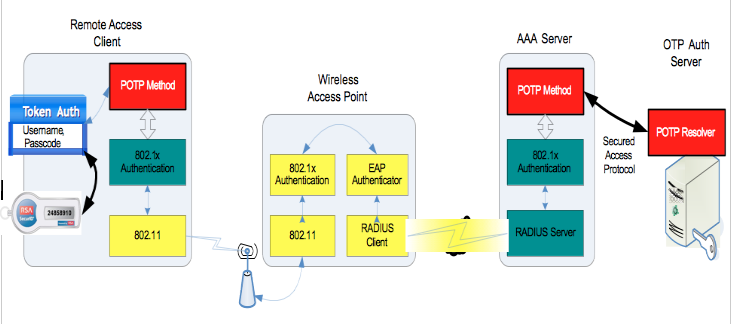
\includegraphics[width=400pt]{image2.png}
  \caption{schéma du matériel token-client-serveur}
  \label{fig:image}
\end{figure}

\section{Approfondissement}

\subsection{Format d'un paquet EAP-POTP}

\begin{tabular}{  l  l  }
	bit 1 &: Code (1 si demande, 2 si réponse)\\
	bit 2 &: Identifier (Permet aux réponses de correspondre aux demandes)\\
	bit 3/4 &: Length (Indique la longueur du paquet entier)\\
	bit 5 &: Type (Spécifie l'algorithme OTP utilisé)\\
	bit 6 &: Reserved (Emplacement réservé pour une future utilisation)\\
	bit 7... &: TLV-based EAP-POTP message \\
\end{tabular}

\subsection{Différent types de TLV}

\begin{description}
   \item \textbf{Type de TLV :}
\item   1 - Version TLV : Contient la version de la méthode EAP-POTP supportée.
\item   2 - Server-Info TLV : Fournit les informations de sessions et des informations sur le serveur.
\item   3 - OTP TLV : Contient des informations sur la procédure d'authentification.
\item   4 - NAK TLV : Indique que le client ne prend pas en charge le paquet reçu.
\item   5 - New PIN TLV : Permet de demander un nouveau code PIN à l'utilisateur.
\item   6 - Confirm TLV : Confirme l'authentification du "peer", le serveur éssaie de s'authentifier auprès du "peer".
\item   7 - Vendor-Specific TLV : Permet l'envoie de plusieurs TLV simultanés.
\item   8 - Resume TLV : envoyé par le client pour tenter la reprise de session.
\item   9 - User Identifier TLV : Donne un identifiant au détenteur du token.
\item 10 - Token Key Identifier TLV : Fournit l'identifiant au token pour qu'il puisse générer un OTP.
\item 11 - Time Stamp TLV : Envoyé par le client pour simplifier l'authentification, fournit le temps du token.
\item 12 - Counter TLV : Envoyé par le client pour simplifier l'authentification, fournit le compteur du token.
\item 13 - Keep-Alive TLV : Envoyé par le "peer" pour éviter les délais d'attente lors de l'attente d'un action utilisateur.
\item 14 - Protected TLV : Chiffre les TLV.
\item 15 - Crypto Algorithm TLV : Permet la négociation de l'algorithme de chiffrement.
\item 16 - Challenge TLV : Fournit le challenge tel que donné par le token.
\end{description}


\subsection{Déroulement type d'une authentification}



Le serveur envoi une EAP-demande type=Identity\\
Le client envoi une EAP-réponse type=Identity\\

Un serveur qui n'utilise pas les algorithmes par défaut (comme SHA256) doit envoyer un Crypto Algorithm TLV dès la première EAP-demande de type POTP-X.\\

\begin{flushleft}
\begin{algorithm}[!h]
	\caption{Serveur}
	\label{POTP:verif}
\begin{algorithmic}
\STATE envoie une EAP-demande avec le type de l'algorithme OTP, la plus haute et la plus basse version de la méthode EAP possible
\STATE l'OTP TLV contient la demande de l'OTP courant
\STATE cette EAP-demande peut potentiellement contenir un chalenge, des informations sur la politique du serveur...
\IF{Cas d'une reprise de session}
	\STATE Server-Info TLV : renvoie l'identifiant serveur et l'identifiant session
\ELSE
	\STATE Server-Info TLV : envoie le nouvel identifiant session
\ENDIF

\end{algorithmic}
\end{algorithm}
\end{flushleft}


\begin{flushright}
\begin{algorithm}[!h]
	\caption{Client}
	\label{POTP:verif}
\begin{algorithmic}
\IF{POTP-X ou la version d'EAP-POTP n'est pas supporté(e)}
	\STATE envoi une EAP-réponse Nak (fin de l'échange)
\ELSE
	\STATE envoi une EAP-réponse avec Version TLV : plus haute version d'EAP-POTP possible entre le client et le serveur
	\IF{la plus haute version est la même pour le Client et le Serveur ET le serveur a envoyé Server-Info TLV dans son EAP-demande}
		\STATE Le peer regarde s'il existe une session sauvegardée
		\IF{Si une session existe ET reprise de session possible}
			\IF{protected mode}
				\STATE le peer calcule les nouvelles clefs de session
			\ENDIF
			\STATE envoie une EAP-réponse avec Resume TLV et Version TLV
		\ENDIF
	\ELSIF{la plus haute version est la même pour le Client et le Serveur ET le serveur a envoyé OTP TLV dans son EAP-demande}
		\STATE le token calcule un nouvel OTP (basé sur les informations de l'EAP-demande)
	\ELSIF{la plus haute version n'est pas la même pour le Client et le Serveur OU le serveur n'a pas envoyé de Version TLV}
		\STATE le peer envoie juste Version TLV dans son EAP-réponse
	\ENDIF
\ENDIF

\end{algorithmic}
\end{algorithm}
\end{flushright}


\begin{flushleft}
\begin{algorithm}[!h]
	\caption{Serveur}
	\label{POTP:verif}
\begin{algorithmic}
\IF{$EAP-réponse = Nak TLV$}
	\STATE la négociation a échoué
	\STATE le serveur peut tenter une autre méthode EAP
\ENDIF
\IF{c'est une reprise de session et le numéro de session est mauvais}
	\STATE le serveur indique au client que la reprise de session et impossible
	\STATE le serveur demande un nouvel OTP
\ENDIF
\IF{EAP-réponse type POTP-X est vide}
	\STATE envoie EAP-échec
\ENDIF
\IF{Authentification possible}
	\STATE accepte authentification
	\STATE envoie EAP-demande avec un Confirm TLV
	\IF{EAP-demande nécéssaire}
		\STATE Le serveur passe en état protégé : tous les POTP-X TLV suivants seront chiffrés et auront leur intégrité protégée
	\ENDIF
\ELSE
	\STATE échec de l'authentification
	\STATE envoi EAP-failure
\ENDIF

\end{algorithmic}
\end{algorithm}
\end{flushleft}



\begin{flushright}
\begin{algorithm}[!h]
	\caption{Client}
	\label{POTP:verif}
\begin{algorithmic}
\IF{EAP-demande de notification}
	\STATE le client tente d'authentifier le serveur
	\IF{le serveur a bien été authentifié}
		\STATE envoi d'une EAP-réponse de type POTP-X avec un Confirm TLV
	\ELSE
		\STATE envoi une EAP-réponse de type POTP-X vide
	\ENDIF
\ENDIF

\end{algorithmic}
\end{algorithm}
\end{flushright}


\begin{flushleft}
\begin{algorithm}[!h]
	\caption{Serveur}
	\label{POTP:verif}
\begin{algorithmic}
\IF{EAP-réponse type POTP-X est vide}
	\STATE envoie EAP-échec
\ENDIF

\end{algorithmic}
\end{algorithm}
\end{flushleft}


\subsection{Reprise de session}
La reprise de session utilise des identifiants de session et des identificateurs serveur pour permettre plusieurs authentifications à la suite.
Pour une reprise de session le serveur renvoie des informations dans un Serveur-Info TLV qui est utilisé par le client pour reprendre la session.
Le peer puis le serveur décident de poursuivre ou pas la session (attention : la session ne doit pas durer plus longtemps que le temps nécessaire pour trouver l'OTP).
Le wifi est particulièrement concerné par cette fonctionnalité.

\subsection{Mode Protégé}
"MAC" (algorithme MAC négocié) est l'algorithme utilisé en mode protégé pour l'authentification et la garantie d'intégrité des données.
Il est calculé comme suit : \\
$mac = MAC(K\_MAC, msg_hash(msg_1, msg_2, ..., msg_n))$\\
Il est possible pour des questions d'économie d'espace de stockage de ne hacher que partiellement le message.\\


Lorsque le mode protégé est activé (en fixant le bit P dans OTP TLV), l'OTP peut être combiné à d'autres informations:\\

Pour la technologie HMAC on se réfère aux précédentes présentations.\\
PBKDF2 = password-based key derivation functions\\
SHA-256 = algorithme de hachage\\
$PBKDF2(otp,salt,pepper,authData,iteraction_count,Key Length) = K_MAC.K_ENC.MSK.EMSK$\\


$K\_MAC$ : clé MAC utilisée pour l'authentification et l'intégrité mutuelle\\
$K\_ENC$ : clé de cryptage utilisée pour protéger certaines données au cours de l'authentification\\
SRK : clé de reprise de session utilisée uniquement pour la reprise de session\\
MSK : clé de session maître\\
EMSK : clé de session maître étendue\\
salt : valeur envoyé en clair\\
pepper : utilisation précisée par le système. Génération aléatoire d'une séquence qui ne sera pas envoyé au serveur mais dont la taille sera envoyée au serveur. Ceci ralentira le haché, encore qu'on a une validation d'otp valide dans le temps.\\

Non envoyé en clair : OTP et pepper

\begin{figure}[!h]
  \centering
  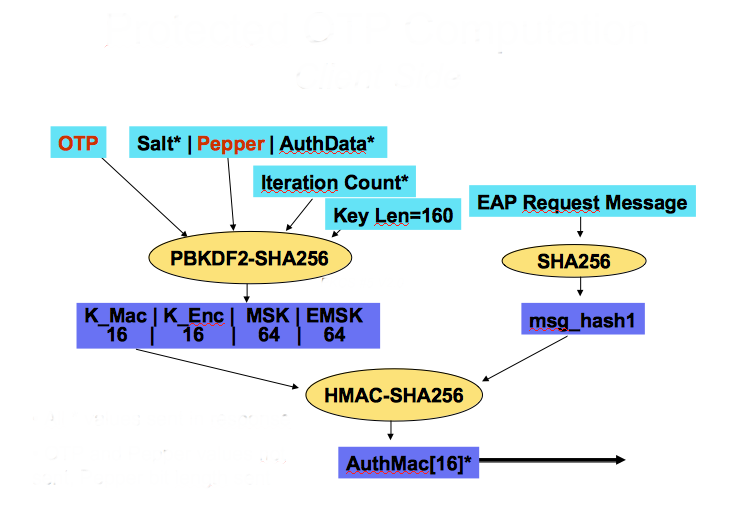
\includegraphics[width=400pt]{image3.png}
  \caption{Mise en place du mode protégé}
  \label{fig:image}
\end{figure}

\section{Analyse générale et sécurité}

\subsection{Avantages et intérêts}
  Cette méthode inclut un grand nombre d'algorithmes OTP.
  Elle permet aussi bien une authentification mutuelle que unilatérale.
  Le mode protégé protège contre les attaques par rétrogradation de versions (version downgrade attacks) ainsi que beaucoup d'autres attaques.\\
  L'utilisation du poivre permet une meilleure sécurité pour un coût initial plus élevé mais égal sur le long terme.
  Il ralentit l'attaquant dans sa recherche du bon OTP.\\
  
  Bien qu'il soit possible d'accéder à l'application de façon indésirable et donc de monter une attaque man-in-the-middle, cela ne compromet pas MSK et EMSK ce qui protège une session ultérieure.
  
  \subsection{Inconvénients et limites}
  Un poivre choisit par le client peut être plus simple à trouver par un attaquant, car potentiellement plus court.\\
  L'utilisation d'un tunnel sécurisé est nécessaire pour offrir une meilleure sécurité au système.\\
  Beaucoup d'attaques restent possibles même si on connait les moyens pour les contrer.

\subsection{Considérations de sécurité}

\subsubsection{Attaques exhaustives (Brute-Force)}
    La session doit durer moins longtemps que le temps nécessaire à une attaque exhaustive, afin que celle-ci n'aboutisse pas.\\
Une autre façon de se protéger contre cette attaque est de hacher un grand nombre de fois avec la fonction PBKDF2.
On peut aussi intégrer un poivre (ou "pepper") dans le hachage (Par contre, si le poivre est partagé dans un Confirm TLV ultérieur, il doit être plus long que celui choisit initialement et chiffré avec PBKDF2).

\subsubsection{Attaque de course (Race Attack)}
Dans la variante de base, il est parfois possible d'écouter plusieurs OTP.
Il faut donc empêcher la création simultanée de plusieurs sessions. (Il existe d'autre façon de contrer cette attaques).

\subsubsection{hijacking taking}
La variante de base est vulnérable au détournement de session (après authentification), mais pas la variante protégée.

\subsubsection{attaques par rejeu (replay attack)}
La variante de base est vulnérable aux attaques par rejeu : l'attaquant peut rejouer une demande (valide) précédente, il peut aussi se servir du code PIN qui est, dans cette variante, transmit sans protection.
Le peer ne doit donc utiliser la variante de base que lorsque le serveur est authentifié et la connexion sécurisée.

\subsubsection{Denial-of-service}
 Les attaques par déni de services sont possible, il faut donc que le serveur ne tienne pas compte des OTP TLV avec un trop grand nombre d'itérations.
Ces attaques ralentissent le serveur.

\subsection{Failles connues}
    Un ancien OTP permet de trouver certaines informations sur le PIN de l'utilisateur et représente donc toujours un risque (il faut donc s'assurer que le PIN de l'utilisateur change régulièrement).\\

   \textbf{ Pour la version avancée:}
    Protection par la variante de la méthode EAP : temps limité d'une session afin d'éviter que l'attaquant (man-in-the-middle) aie le temps de trouver l'OTP valide.\\
    
    \textbf{Pour la version de base:}
    Une attaque par man-in-the-middle est possible (il faut être en authentification mutuelle pour s'en protéger).
    Détournement de session et attaques par rejeu (pour s'en protéger il faut être connecté de façon sécurisée à un serveur authentifié, en utilisant PEAPv2 par exemple).
    Lors de la reprise de sessions (en canal sécurisé) il reste possible de trouver la combinaison identifiant de session/OTP (pour s'en protéger il faut garder une trace du nombre de tentatives infructueuses de reprises).

\subsection{Précautions et préconisations}
    Dans le cas d'une reprise de session, celle-ci doit durer moins longtemps que le temps nécessaire pour trouver l'OTP utilisé.\\
    La version de base comporte de nombreuses failles, il vaut mieux utiliser la variante protégée (protected variante).\\
    Le poivre doit être stocké de façon sure.\\
    Les informations sensibles doivent être envoyées par un tunnel sécurisé.\\
    
    Pour la variante de base, lors d'une reprise de session (dans un tunnel sécurisé) il reste une probabilité de $1/2^48$ qu'une attaque réussisse en trouvant le couple identifiant de session/valeur de l'OTP. Le serveur doit donc garder une trace du nombre de tentatives de reprise de session infructueuses.\\

\section{Conclusion}

  \subsection{Utilisation dans le cadre du projet}
  La réussite de l'authentification (unilatérale ou mutuelle) grâce aux mots de passes jetables de deux systèmes via le réseau.
  
  \subsection{Pérennité du système}
  La pérennité est au plus égale à celle de la fonction de hachage utilisée.

\section{Définitions}
OTP-X : Désigne une méthode OTP quelconque.\\
Code PIN : Il est composé de caractères UTF-8 (sa longueur dépend de l'application) sans caractère de fin NULL.\\
Poivre ou pepper : Valeur inconnue des tierces personnes (secret partagé) qu'on inclut dans la fonction de hachage.\\
PBKDF2 : password-based key derivation functions.\\
SHA-256 : algorithme de hachage.\\

\end{document}
